\section{模块与功能详细设计}

\subsection{模块总览}

系统由 14 个 NestJS 服务端模块 + 1 个 Mediasoup Worker 子进程 + 9 个前端功能模块组成，以下按服务端模块说明核心职责和关键技术实现。

\subsection{核心功能模块设计}

\subsubsection{用户登录模块}

涉及接口：RegisterUser、LoginUser。关键实体：User、AuthSession。

业务流程：
\begin{enumerate}[itemsep=0pt]
  \item 用户提交注册信息（用户名、邮箱、密码），系统校验唯一性和密码强度，写入 users 表
  \item 登录时查询 users 表验证 bcrypt 密码哈希，验证通过后创建 auth\_sessions 行
  \item 返回 access\_token（JWT 短有效期）+ refresh\_token（长有效期），附带用户/好友/社区/未读/通知快照
  \item 刷新令牌时验证旧 refresh\_token 未过期/未撤销，轮换生成新令牌对；登出时设置 revoked\_at
\end{enumerate}

\subsubsection{消息发送模块}

涉及接口：SendMessage、LoadMessages、MarkRead、DeleteMessage。关键实体：Message、ReadState、MessageAttachment、MessageMention。

\textbf{频道消息流程：}
\begin{enumerate}[itemsep=0pt]
  \item 事务内执行：INSERT messages → INSERT message\_attachments → INSERT message\_mentions
  \item 发送者标记已读（markSenderRead），其他频道成员 unread\_count + 1（incrementChannelUnread）
  \item @提及触发通知创建（NotificationsService.createNotification）
  \item 事务提交后广播 MessageCreated + UnreadUpdated 实时事件
\end{enumerate}

\begin{figure}[H]
\centering
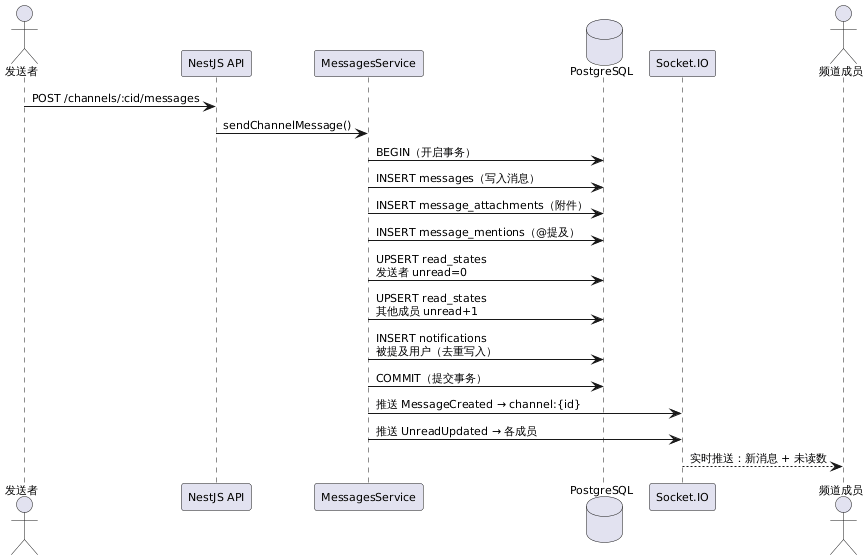
\includegraphics[width=0.80\textwidth]{figures/v1.png}
\caption{频道消息发送事务流程}
\label{fig:msg-channel}
\end{figure}

\textbf{DM 私聊流程：} 同上，区别在于关联 direct\_conversations，仅对接收方 +1 未读，并创建 direct\_message 通知。

\begin{figure}[H]
\centering
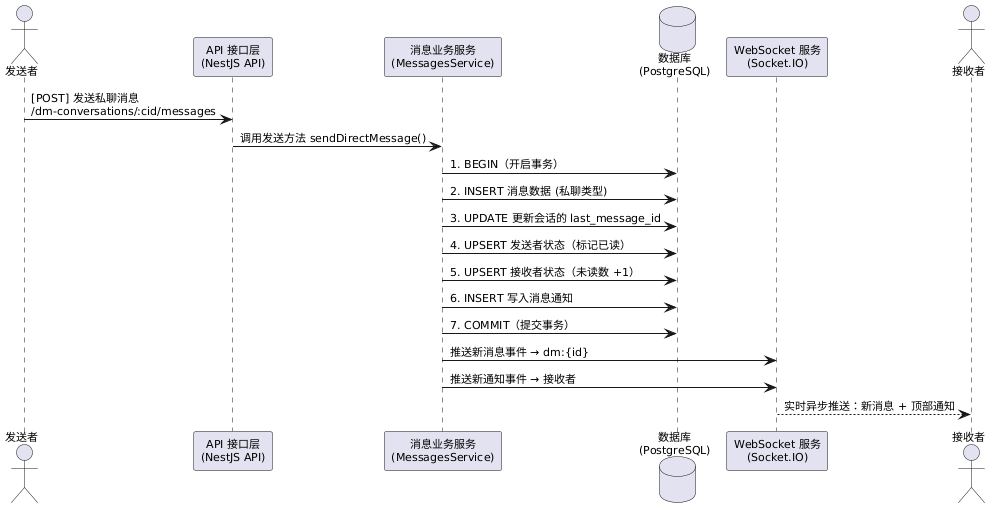
\includegraphics[width=0.75\textwidth]{figures/dmflow.png}
\caption{DM 私聊发送事务流程}
\label{fig:msg-dm}
\end{figure}

\textbf{消息去重机制：} 通过 \texttt{(senderId, channelId/conversationId, clientMessageId)} 唯一约束防重复。发送前先查询已有消息，存在则直接返回。

\textbf{游标分页加载：} 以 (created\_at DESC, id DESC) 排序，返回 pageLimit + 1 条判断是否有下一页，next\_cursor 编码为 base64url。

\subsubsection{语音通信模块}

涉及接口：JoinVoiceChannel、UpdateVoiceState、LeaveVoiceChannel。关键实体：VoiceSession。

\begin{enumerate}[itemsep=0pt]
  \item 用户 POST join → 创建 VoiceSession → MediaSignaling.prepareRouter 获取/创建 Mediasoup Router
  \item 创建 WebRTC Transport（send + recv），返回 ICE/DTLS 参数 + TURN 凭证（HMAC-SHA1 签名）
  \item 客户端创建 mediasoup-client Transport 完成 DTLS 握手，发送方创建 Producer（kind=audio）
  \item 服务端为收听方创建 Consumer，状态变化广播 VoiceStateChanged
  \item 协商超时机制：超出 negotiationDeadline（$\sim$30s）自动清理僵死会话
  \item Mediasoup Worker 崩溃时 RouterRegistry 标记 Router 失效，客户端需重新 join
\end{enumerate}

\begin{figure}[H]
\centering
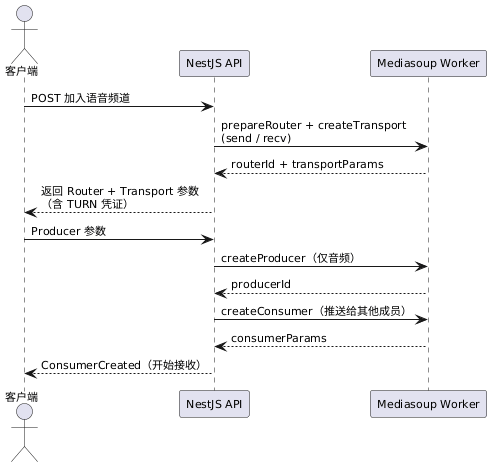
\includegraphics[width=0.78\textwidth]{figures/voice.png}
\caption{WebRTC 语音信令流程}
\label{fig:voice}
\end{figure}

\subsubsection{权限管理模块}

涉及接口：CheckPermission、AssignRole。关键实体：Role、PermissionOverwrite、MembershipRole。

\textbf{权限模型：} bitmask 组合。Owner（全权限）$\to$ 角色权限并集 $\to$ 频道覆盖（allowBits / denyBits）。

权限位定义：
\begin{center}
\begin{tabularx}{\textwidth}{L{3cm}L{3cm}Y}
\toprule
\textbf{权限} & \textbf{位值} & \textbf{说明} \\
\midrule
ViewChannel & 1 & 查看频道 \\
SendMessage & 2 & 发送消息 \\
ManageMessage & 4 & 管理消息（删除）\\
ManageChannel & 8 & 管理频道 \\
JoinVoice & 16 & 加入语音频道 \\
ManageMember & 32 & 管理成员 \\
ManageRole & 64 & 管理角色 \\
CreateInvite & 128 & 创建邀请 \\
ViewAudit & 256 & 查看审计 \\
SpeakVoice & 512 & 语音发言 \\
ListenVoice & 1024 & 收听语音 \\
\bottomrule
\end{tabularx}
\end{center}
默认成员权限 = ViewChannel $|$ SendMessage $|$ JoinVoice $|$ SpeakVoice $|$ ListenVoice（= 1555）。

\subsubsection{实时事件模块}

技术实现：Socket.IO 4.7 网关，房间命名规则：
\begin{itemize}[itemsep=0pt]
  \item \texttt{user:\{id\}} --- 用户私有推送
  \item \texttt{server:\{id\}} --- 社区公告
  \item \texttt{channel:\{id\}} --- 频道公告
  \item \texttt{voice:\{id\}} --- 语音事件
\end{itemize}

核心事件类型（20 种）：MessageCreated, MessageDeleted, UnreadUpdated, NotificationCreated, PresenceChanged, MemberJoined, MemberChanged, ChannelChanged, PermissionChanged, VoiceMemberJoined/Left, VoiceStateChanged, VoiceRouterCapabilities, VoiceTransportCreated/Connect, VoiceProducerCreated, VoiceConsumerCreated/Resumed, VoiceProducerClosed, VoiceActiveSpeaker, SyncState。

断线重连后客户端发送 SyncState 全量同步当前状态。

\subsubsection{前端架构}

采用 React 18 + Vite + TypeScript SPA，9 个功能模块：auth, servers, channels, messages, voice, friends, notifications, permissions, profile。共享组件 17 个（AppShell, ServerRail, MessageList, MessageComposer, VoiceStrip 等）。状态管理使用 Zustand（auth-store, workspace-store, toast-store）+ React Query（服务端数据缓存/失效/重取）。